\chapter{Simulation}\label{chap:sim}
	The data collected by the \gls{ATLAS} experiment must be compared to a well understood dataset. This dataset is most often a dataset of simulation particle collisions that aim to mimic physics processes and particle interaction with detector material, as well as the detector's response. Figure \ref{fig:simulation} shows the chain of simulations by which these datasets are produced.
	\begin{figure}[!ht]
	\centering
	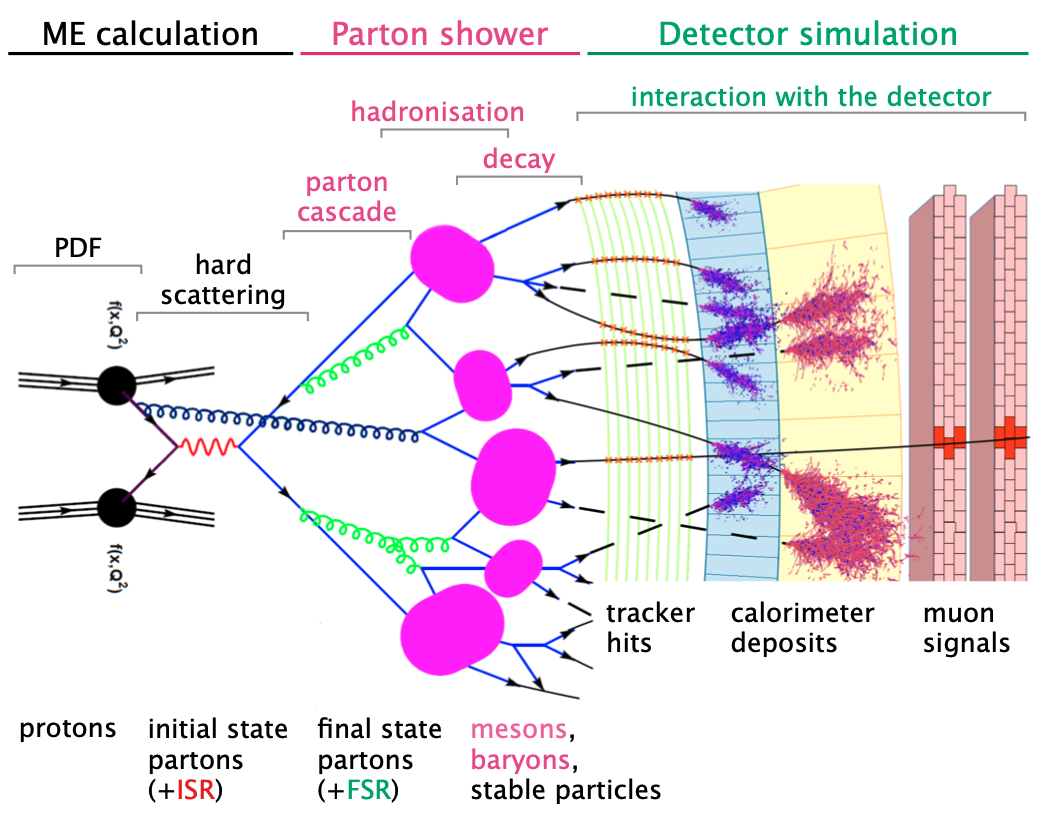
\includegraphics[width=.95\textwidth,keepaspectratio=true]{chapters/chapter4_simulation/images/Simulation_Chain.png}
	\caption{\label{fig:simulation} A pictorial representation of the simulation chain used in the \gls{ATLAS} experiment \cite{Wanotayaroj:2242196}.}
	\end{figure}
	
	Many particle physics experiments, \gls{ATLAS} included, use \gls{MC} simulation techniques to produce these datasets. Monte Carlo simulation techniques use repeated random sampling of underlying probability density functions to closely model various processes. 

	\section{Event Generation and Hadronization}\label{sec:event-gen}
		Since protons and other hadrons are not fundamental particles, it is impossible to know the exact constituents (partons) that interacted during a collision. To mimic this intrinsic probabilistic nature, \acrfullpl{PDF} are used. A \gls{PDF} models the probability of any parton within a proton (or hadron) to carry a fraction of the beam energy at a given hadron momentum. The \gls{PDF} and subsequent inelastic hard scattering of the interacting partons are modeled via a \gls{ME} calculation, which can be depicted through Feynman diagrams. This \gls{ME} calculation is done to fixed order in perturbation theory, \gls{LO}, \gls{NLO}, \gls{LL}, etc. This first level event generation can be done by a myriad of \gls{MC} event generators. Often specific choices are made based on individual generator performance for a given physics process.

		The next step in the simulation chain is the parton showering and hadronization. This can be done with a different set of \gls{MC} simulations. Parton showering and hadronization are complex, computationally expensive steps to simulate and are done iteratively. An example of a parton shower generator output can be seen in Figure \ref{fig:hadronization}.

		The \gls{MC} generators used in this dissertation for background simulations are Pythia \cite{pythia}, Powheg-Box \cites{powheg-1}{powheg-2}, and Sherpa \cite{sherpa}. For signal, MadGraph is used \cite{MadGraph}. For all processes, Pythia8 is used to simulate the parton shower, fragmentation, and underlying event. Table \ref{tab:bkg-generators} shows which \gls{MC} generator is used for each background process.

				\begin{table}[!thp]
			\begin{center}
			\caption{\label{tab:bkg-generators}
			\gls{MC} generators for the main \acrshort{SM} background samples at \sqs used in this dissertation. 
			Here, $\ell$ refers to the three lepton families $e$, $\mu$ and 
			$\tau$.
			}
			\small
			\resizebox{0.75\textwidth}{!}{
			\begin{tabular}{|c||c|}
			\hline
			Background process & Generator \& parton shower  \\
			\hline \hline
			\ttbar with at least one lepton $\ell$ 	& 	Powheg \& Pythia8 	\\ \hline
			Single top-quark 						& 	Powheg \& Pythia8 	\\ \hline
			W ($\ell \nu$) + jets 					& 	Sherpa 				\\ \hline
			Z/$\gamma^{*}(\ell \ell , \nu \nu)$ + jets &Sherpa 				\\ \hline
			$WW$ 									& 	Powheg \& Pythua8 	\\ \hline
			$WZ$ 									& 	Powheg \& Pythua8 	\\ \hline
			$ZZ$ 									& 	Powheg \& Pythua8 	\\ \hline

			\end{tabular}}
			% \normalsize
			\end{center}
		\end{table}

		\begin{figure}[!ht]
		\centering
		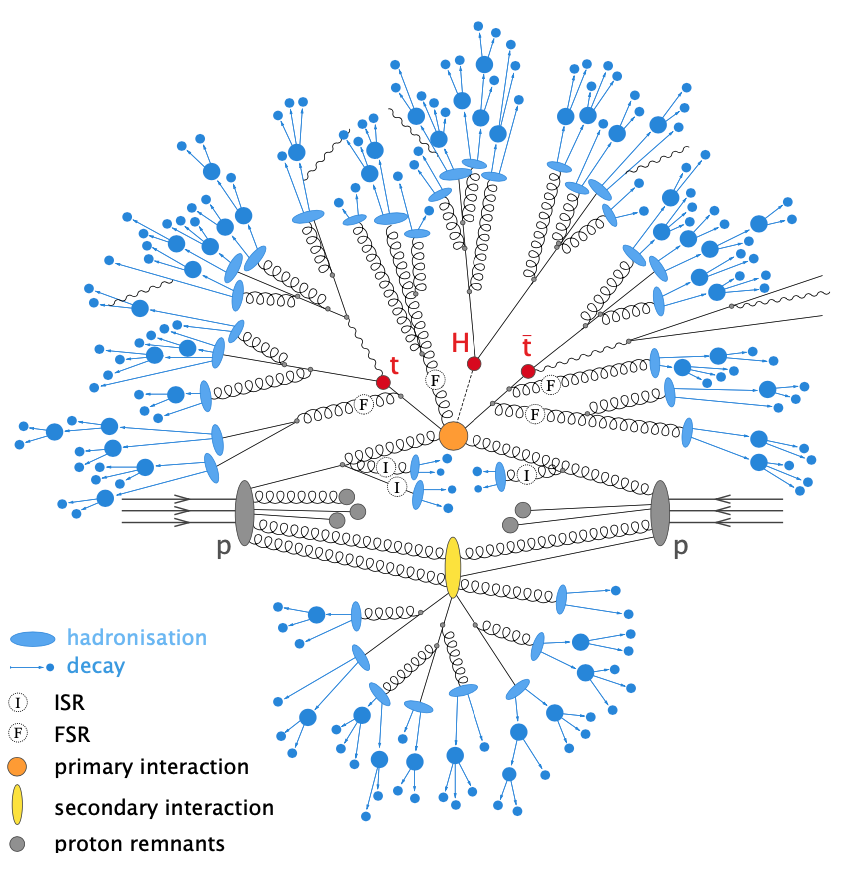
\includegraphics[width=\textwidth,keepaspectratio=true]{chapters/chapter4_simulation/images/tth_hadronization_gen.png}
		\caption{\label{fig:hadronization} A pictorial representation of a parton shower of a t$\bar{\mathrm{t}}$H event \cite{Wanotayaroj:2242196}.}
		\end{figure}	

	\section{Detector Simulation}\label{sec:detector-sim}
		The final step in the simulation chain is simulating the particle's interaction with the detector material and the detector's response. Up until this point, the \gls{MC} generators used are generic non-experiment dependent simulations. The \gls{ATLAS} collaboration uses a GEANT4 based generator suite to simulate these interactions \cite{GEANT4}. These detailed simulations include all support structure, material densities, readout electronics, and digitization in order to fully simulate the path of a real particle through the \gls{ATLAS} detector. These simulations are often too slow to produce enough statistics for physics analyses. In the full simulation, around $80\%$ of the simulation time is spent on particles traversing the calorimeters and $75\%$ is spent on electromagnetic particles alone \cite{ATLAS-simulation}. Instead, several methods were developed to speed up the simulation known as FAST simulations. A detailed description of the \gls{ATLAS} simulation chain and options can be seen in Reference \cite{ATLAS-simulation}. The final simulated dataset is output into a raw data format identical to real data coming off of the \gls{ATLAS} detector. 

		